Analysis of events occurring in the range of femtoseconds is desired in many scientific experiments.
The high temporal resolution needed for measuring such events imposes a great technological challenge for \glspl{daq} and \glspl{adc}.
In order to relax the requirements on the acquisition systems, the so-called optical time-stretch technique is used to stretch the analog input signal in time.
In this way, data converters at relatively moderate sample rate can be used.
Measuring the signal with commercial \glspl{daq}, such as real-time oscilloscope, still poses another challenge.
Due to the limited acquisition time windows of such systems, continuous measurements at high sampling rate over long time is not possible.
In applications, where measurements of long-term evolution of the ultra-fast events is desired, this is a major limitation.
Therefore new concepts of \gls{daq} based on the time-stretch method need to be considered in order to overcome this limitation. 

In this thesis, a first demonstrator of such a new \gls{daq} system based on the photonic time-stretch method was developed.
The system consists of a high bandwidth front-end sampling card, mounted on a back-end card integrating a new generation of \gls{rfsoc} for readout of the acquired samples. The name given to the system is \gls{theresa}.

The front-end sampling card integrates 16 sampling channels, each containing a \gls{tha} with individually programmable delay in sampling time. 
The design of the board allows it to be used in two different modes: with and without the time-stretch setup.
In single-channel mode one detector is connected to one sampling channel, therefore allowing sampling of up to 16 detectors at the same time with one sampling point per channel.
In the second mode, several channels are connected to one detector via power splitter, therefore allowing multiple sampling points for one detector/per channel by setting the delay times accordingly. 

High-speed \glspl{adc}, integrated in the \gls{rfsoc}, with 14-bit resolution and a sample rate of up to \SI{2.5}{\giga \sample \per \second} allow continuous sampling of the signal with high time resolution. 
Using the time-interleaving technique for all sixteen \glspl{adc} results in an overall maximal achievable sample rate of \SI{40}{\giga \sample \per \second} possible.  
When using in combination with the time-stretch technique and considering typical stretch-factors, these \SI{11}{\pico \second} are translated into a range of femtoseconds in the original signal.

The sampling card was furthermore designed to fully exploit all the features of the \gls{rfsoc}, which integrates a processing unit together with a \gls{fpga}.
An evaluation tool framework is provided for the selected read-out card, allowing for on-board data generation and capture.
This tool was also evaluated; allowing for quick set-up and measurement of key data converter characteristics (\gls{sinad}, \gls{sfdr}, ...) it provides an invaluable tool in order to get a first impression of the performance of the sampling card.

The on-chip \gls{fpga} provides the possibility to flexibly adjust the firmware to user needs. 
Slow-control implemented in the \gls{fpga} takes care of programming the components on the sampling card, such as the delay chips.
High-speed interfaces, allowing speeds over 100 Gb/s, are a crucial component for the high throughput of the large amount of data generated by the data converters; with the given resolution and max. sample rate this touches the range of TB/s.


The design of the sampling card was approved and the card has been deployed in production.
Quick characterization of the card is possible due to the tool provided for the redout-card and can be carried out using the methods described in \autoref{ssec:adc_charac}.
\gls{theresa} will then be commissioned and taken into operation, improving the research in various scientific fields, especially beam diagnostics at e.g. \gls{kara}. 
There it can be used for studying \gls{csr}, in the far-field and near-field electro-optic setup, for study of fast laser dynamics and many other applications.
The selected \gls{fpga} is suitable for deploying Artificial Intelligence applications (i.e. Reinforcement Learning).
Therefore the system can also be used for interfacing with the Bunch-By-Bunch feedback at \gls{kara}.
In the context of the ULTRASYNC project, funded by ANR-DFG, \gls{theresa} can be used in order to study the control of electron bunches in accelerators at \gls{kara} and SOLEIL, therefore being an important step towards new usable \gls{thz} sources. 
 

%There is a disturbing lack of benches in \sout{Ramset Park} Campus North. I want to sit more!
%
%\begin{figure}[tbh]
%	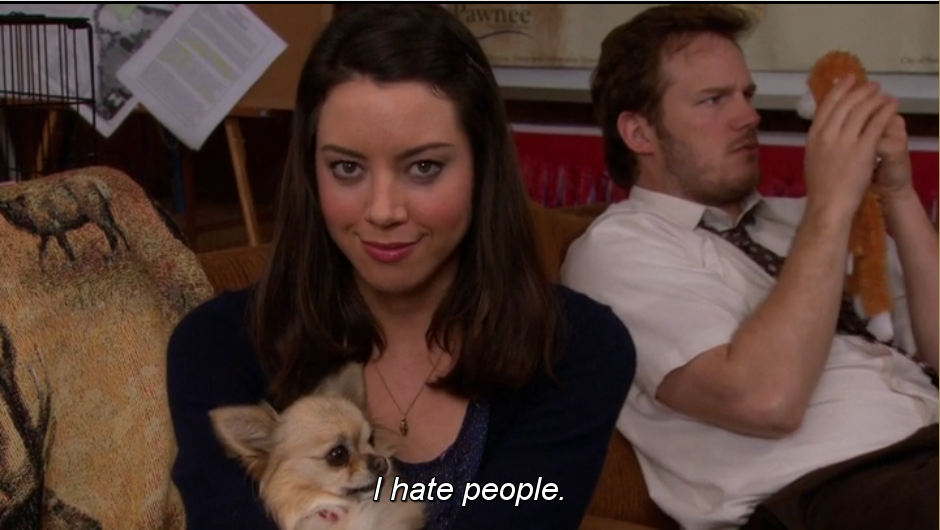
\includegraphics[width=\textwidth]{chap/06-conclusion/img/april}
%\end{figure}
%
%\newpage
%\section{Expectation vs. Reality}
%At least I wrote more than 273 words.
%\begin{figure}[tbh]
%     \centering
%     \begin{subfigure}{0.7\textwidth}
%         \centering
%         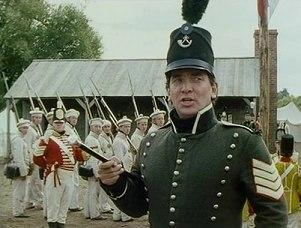
\includegraphics[width=\textwidth]{chap/06-conclusion/img/harper}
%         \caption{How you think you will feel like at the end of your master studies.}
%         \label{fig:expectation}
%     \end{subfigure}
%     
%     \begin{subfigure}{0.7\textwidth}
%         \centering
%         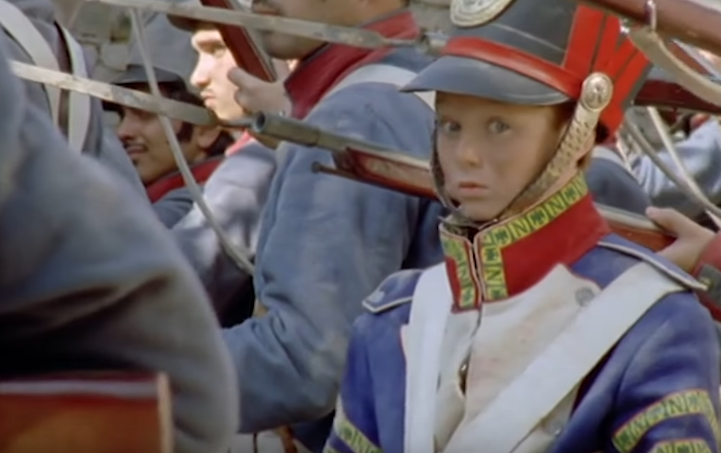
\includegraphics[width=\textwidth]{chap/06-conclusion/img/bubi}
%         \caption{How you actually feel like.}
%         \label{fig:reality}
%     \end{subfigure}
%     \caption{Expectation vs. Reality}
%\end{figure}
%
%
%
%\section{The board}
%\begin{figure}[H]
%	\centering
%	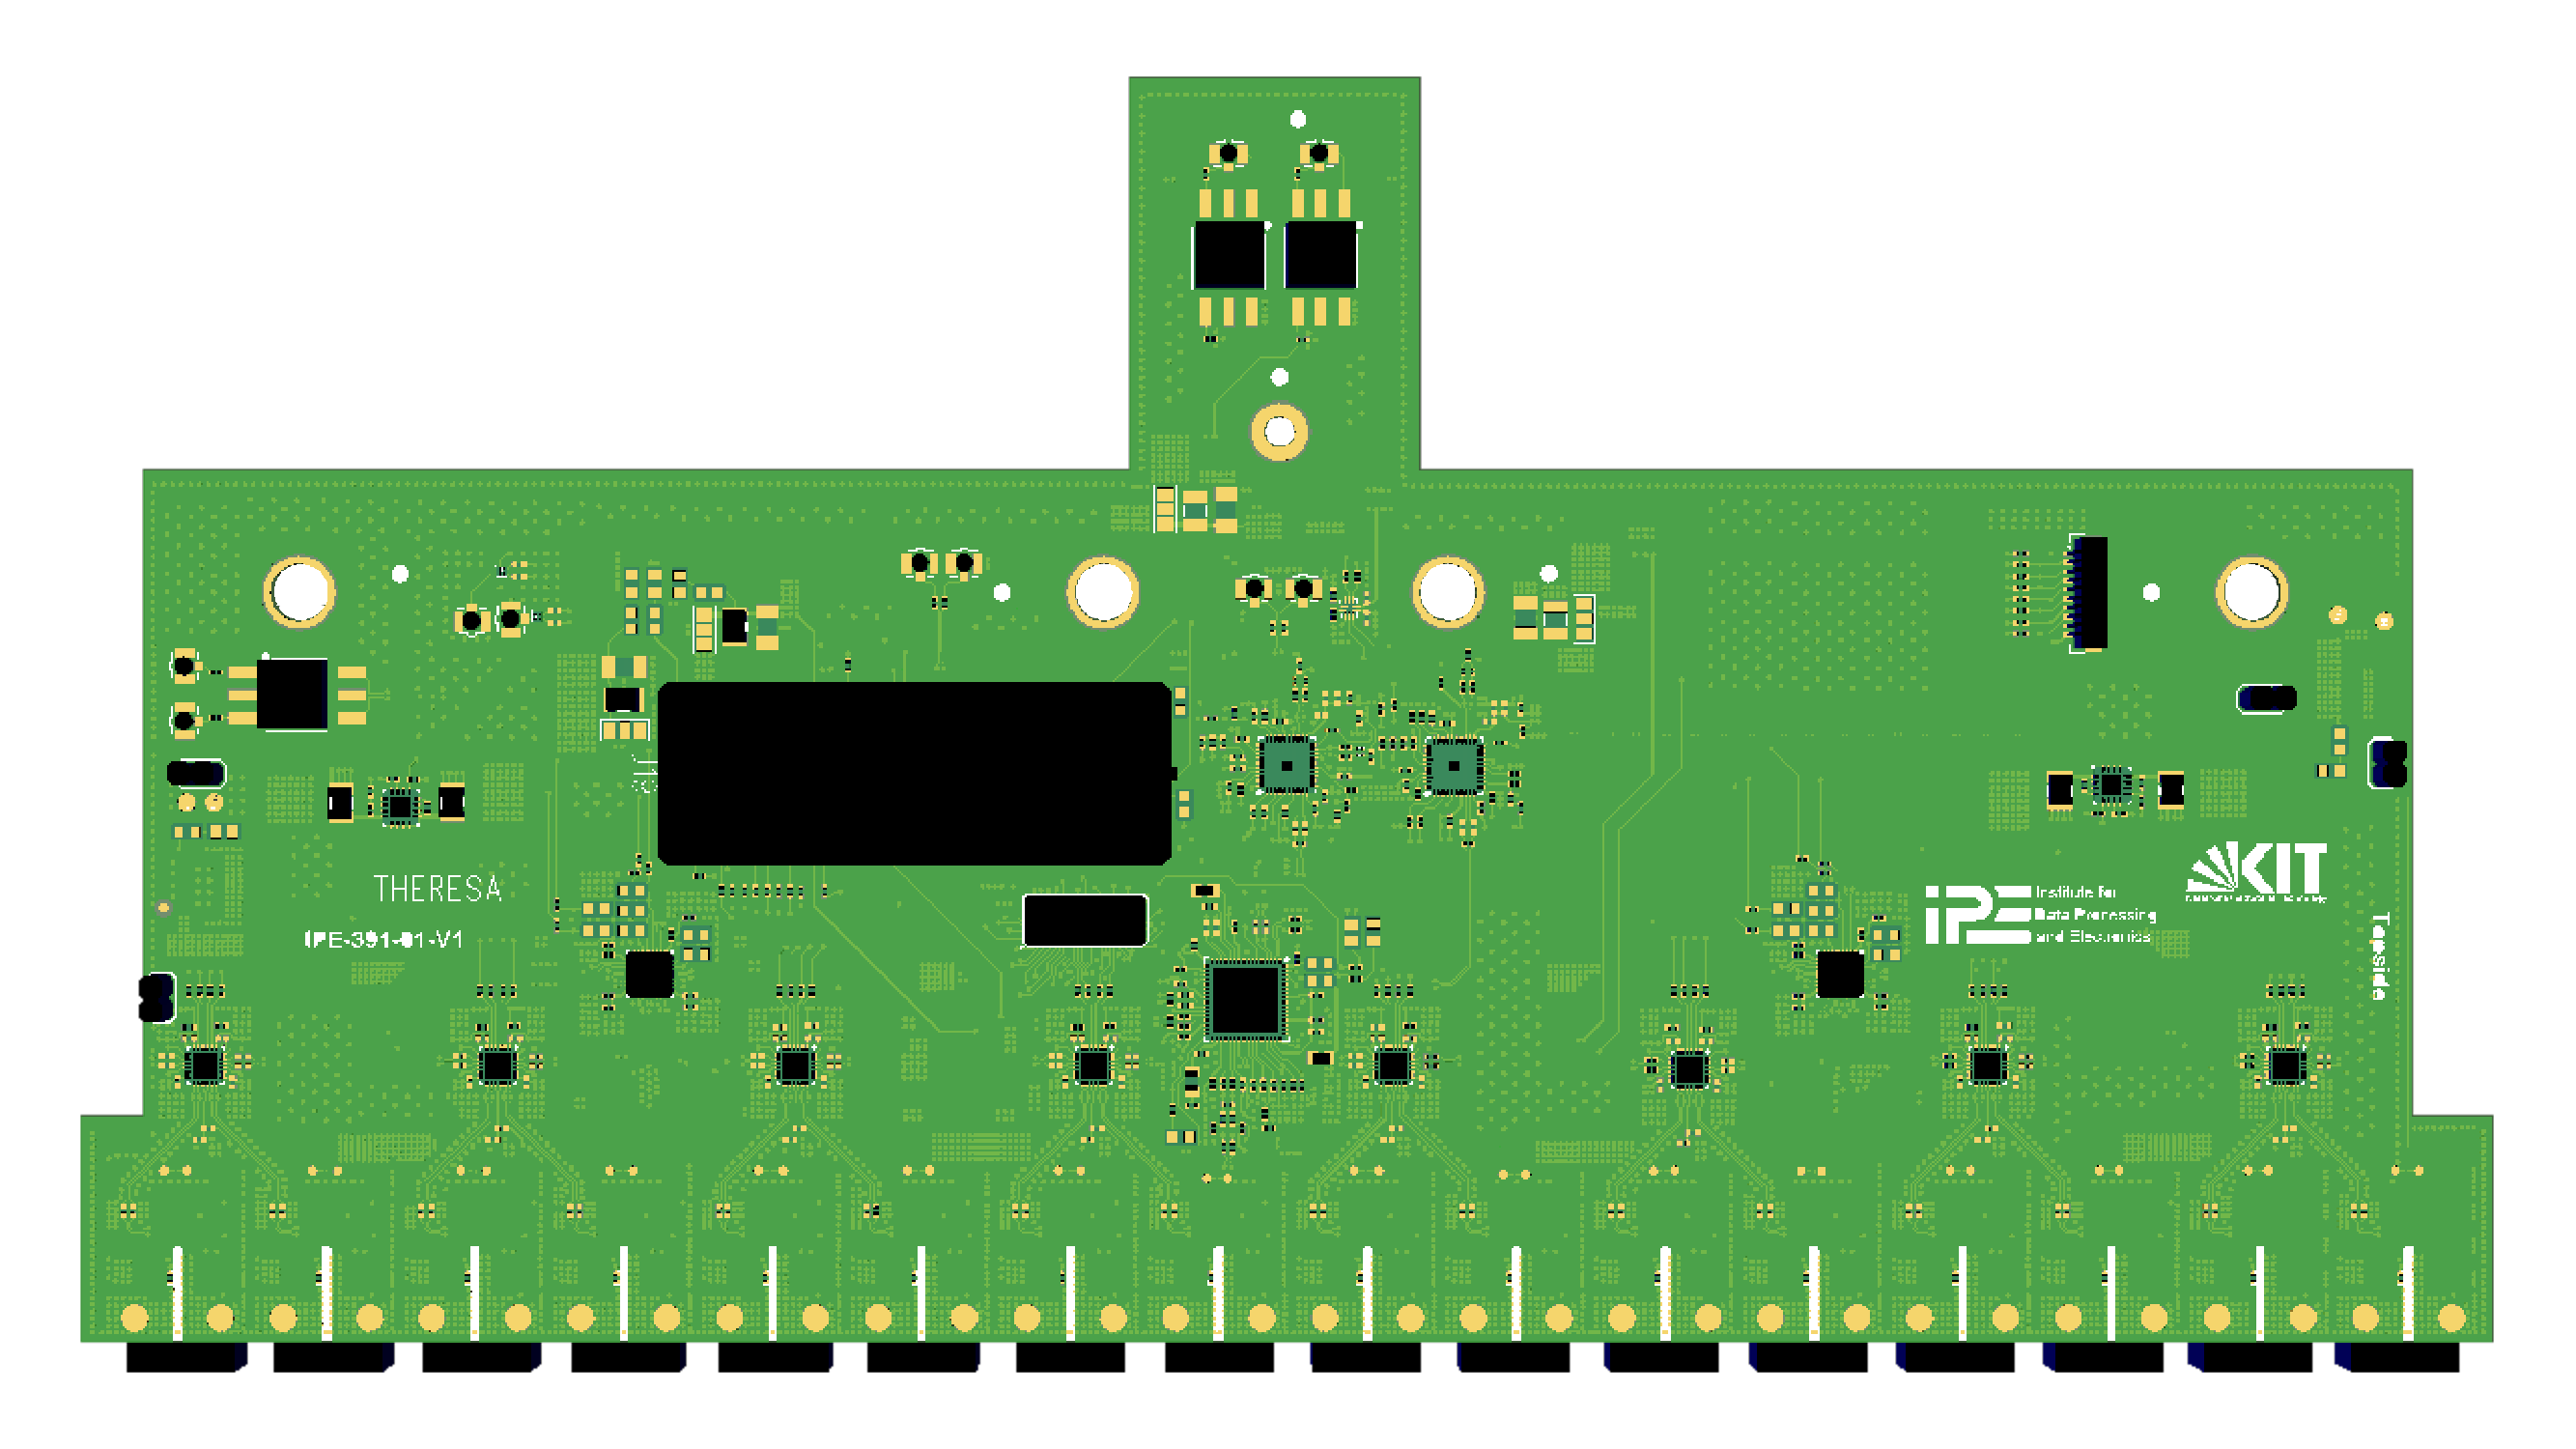
\includegraphics[width = \textwidth]{chap/06-conclusion/img/board}
%	\caption{THERESA}
%	\label{fig:board}
%\end{figure}
